\chapter{Requirement analysis}\label{chapters:analysis}

This chapter summarizes the expectations for the application in the form of requirements. The requirements are analyzed, and in the following chapter, the solution is proposed with a focus on a formal description of the framework.

\bigskip

As \textbf{stakeholders}, we would consider data analysts, programmers, or at least individuals interested in the area of data modeling, since the typical use case of the application is (i) to design schemas for a large system of interconnected subsystems or modules or (ii) to design a recommendation for publishing data. Both these use cases are described in the introduction of this chapter.

Because of the stakeholders' knowledge in the area of data modeling, we may keep the UI of the application more technical as the intent of all operations may be intuitive for them. Nevertheless, the basic functionality does not require advanced knowledge in the abovementioned fields, so we propose an "expert mode." The user will be asked whether they feel like an expert in the area, which would make available more advanced application features while keeping the UI simple for those interested in the basics of data modeling.

\bigskip

\section{General schema}

\begin{requirement}
A user shall be able to easily derive a \textbf{general schema} structure from the existing ontologies and then translate the structure into different known schema languages, such as JSON Schema, XSD, and CSVW Schema and it shall be possible to add support for others easily.
\label{requirement:general-schema}
\end{requirement}

The basic idea behind this requirement was already explained in the Introduction. From an ontology specifying the relations between things from a real world, it should be easily possible to select things and relations between them that describe a schema. The schema then defines a structure of data that represents those things from an ontology.

\begin{figure}[h!]\centering
  \begin{tikzpicture}
      %Nodes
      \node[ontology] (ontology) at (0,0) {Ontology};

      \node[generalSchema] (schema1) at (-3.5,-1.5) {General schema 1};
      \node (psmDot) at (0,-1.5) {...};
      \node[generalSchema] (schemaN) at (3.5,-1.5) {General schema N};

      \node[schema,align=center] (xml1) at (-5.5,-3) {XML\\schema};
      \node[schema,align=center] (json1) at (-3.5,-3) {JSON\\schema};
      \node[schema,align=center] (csv1) at (-1.5,-3) {CSV\\schema};

      \node (psmDot) at (0,-3) {...};

      \node[schema,align=center] (xmlN) at (1.5,-3) {XML\\schema};
      \node[schema,align=center] (jsonN) at (3.5,-3) {JSON\\schema};
      \node[schema,align=center] (csvN) at (5.5,-3) {CSV\\schema};

      %Lines
      \draw[-latex] (ontology) -- (schema1);
      \draw[-latex] (ontology) -- (schemaN);

      \draw[-latex] (schema1) -- (xml1);
      \draw[-latex] (schema1) -- (json1);
      \draw[-latex] (schema1) -- (csv1);

      \draw[-latex] (schemaN) -- (xmlN);
      \draw[-latex] (schemaN) -- (jsonN);
      \draw[-latex] (schemaN) -- (csvN);
  \end{tikzpicture}
  \caption{Diagram showing the core workflow behind the data modeling from an ontology. Users can create general schemas (blue rectangles) from the ontology. From those schemas, the tool creates data schemas in known formats, such as XSD, CSV Schema, or JSON schema.}
\end{figure}

\smallskip

We aim to design a model for a \textbf{general schema} that can describe most of the serialization data formats. This model will be used as a mapping from the ontology to the desired schema. The model must be robust enough to support different formats, as we want to use the same general schema for all of them, which corresponds to MDD as an abstraction layer.

\medskip

There are many formats for data exchange, the most famous being JSON, XML, CSV/TSV, and RDF. Data formats can be categorized into the following categories based on the structure model:
\begin{itemize}
    \item The \textbf{hierarchical model} stores data in a tree-like structure, having one root class with properties that may recursively contain other classes. It has been one of the most common models for data serialization in the past few decades, as it is easy to understand and interpret and is suitable for most types of data. XML and JSON are examples of formats that use this model.
    \item \textbf{Relational model} uses a set of tables to store data. Each table represents a sequence of similar things, each on one row with columns as properties. Rows may point to rows in other tables to link data. The relational model is also famous for its simplicity in CSV and TSV files, which can be easily parsed. The relational model is also used in relational databases (the databases that use SQL query language).
    \item \textbf{Graph model} represents data in a general graph structure with nodes and edges. RDF (Resource Description Framework) became a popular format using the graph model, where nodes usually represent things or literal values, and edges connect them as properties.
\end{itemize}

As our primary intent is to support JSON and XML, we will use the first type of model to represent the data in our general format. The translation from that format to individual schemas in the hierarchical model would be implicit (and will be described later in the text).

Supporting translation from the general schema, which is in the hierarchical model, to the formats in the relational and graph models should be possible in a limited way\footnote{That means we may not be able to reverse translation from specific schema to the general schema or it may not be possible to use the full power of the given specific schema. However, this is not important to us, as our target is the support of basic use cases.}, which is sufficient and follows the requirement to have one general schema.

The graph model is not even necessary to generate as we use the ontology that is already in the graph model; hence, we can use the ontology directly as the schema to validate our data.

%==============================================================================%
\subsection{Analysis of the formats}

We will analyze the standard formats to properly design a user interface for the schema modeling and the underlying general schema model capable of describing those formats.

\smallskip

\textbf{JSON (JavaScript Object Notation)} is a simple format with two complex data types: objects and arrays. The objects represent data in key-value pairs with values that can have any type, including other objects and arrays. Arrays then represent lists, and both arrays as objects may be in the root of the document tree. Semantically, objects represent things with their values as properties.

\textbf{XML (Extensible Markup Language)} is similar to JSON since both formats are hierarchical. XML tags wrap parts of the document representing either things or properties of things and can be nested similarly to the JSON format. In contrast to JSON, XML tags can have attributes.

\begin{figure}[h!]\centering
    \begin{subfigure}[b]{.45\textwidth}
\begin{Verbatim}[commandchars=\\\{\}]
\{
  "id": 3758,
  "title": "Chair",
  "variants": [
    \{
      "title": "Black",
      "price": 200,
      "color": "black"
    \},
    \{
      "title": "White",
      "price": 200,
      "color": "white"
    \}
  ]
\}
\end{Verbatim}
        \caption{JSON document - braces {\tt\{\}} wraps object and brackets {\tt[]} wraps array}
      \end{subfigure}\hfil%
      \begin{subfigure}[b]{.45\textwidth}
\begin{Verbatim}[commandchars=\\\{\}]
<Good id="3758">
  <title>Chair</title>
  <Variant>
    <title>Black</title>
    <price>200</price>
    <color>black</color>
  </Variant>
  <Variant>
    <title>White</title>
    <price>200</price>
    <color>white</color>
  </Variant>
</Good>
\end{Verbatim}

\vfill

        \caption{XML document - {\tt<Good>} tag serves as a class wrapper, whether {\tt<title>} has a property meaning}
      \end{subfigure}
    \caption{Comparison of JSON and XML format both showing data about the same chair.}
    \label{analysis/xml-json}
\end{figure}

As seen in \autoref{analysis/xml-json}, the XML format is more complex, as it supports tag attributes (see \verb|id="3758"| attribute), and arrays can be written in two distinct ways. We can place elements of the array directly in the parent container, as we can see with the \verb|<Variant>| tag, or we can wrap them into another container for clarity (for example, into \verb|<variants>| tag).

\smallskip

JSON Schema is a JSON document that describes the data structure we can expect from other JSON documents. For this part of the thesis, it is sufficient to know that the schema defines which root object we can expect and a set of allowed properties and their types for each object.

Suppose that we have chosen a structure very similar to JSON Schema to be our general structure format. We are interested only in how it describes the document's structure, not its representation. Because JSON is simpler than XML, we can use our model to describe only simple XML documents, as we are missing constructs that would describe advanced XML features.

For example, the object property \textit{x} with primitive value \textit{y} would represent an XML tag {\tt <x>y</x>}; if {\tt y} is an object, we will apply this rule recursively.
The object property \textit{x} with an array of \textit{y\textsubscript{i}}  would represent multiple XML tags {\tt<x>y\textsubscript{1}</x><x>y\textsubscript{2}</x>...<x>y\textsubscript{n}</x>}.
Finally, we will start with the root tag, which was {\tt <Good>} in our case.

To describe and distinguish between more advanced XML features, we would need to add XML-specific options to our model, such as:
\begin{enumerate}
  \item For every object property with a primitive value, there should be an option that the given property becomes an attribute of the parent tag. For example, the \verb|id| property of the chair may be either the attribute \verb|id="3758"| of the parent or the full tag \verb|<id>3758</id>| inside the parent.
  \item For every array property, there should be an option that the given list of tags will be wrapped.\footnote{This may not be necessary as we can add the wrapper class to the general schema by ourselves. This, however, is not the correct solution as the meaning of the wrapper class is not semantical, but rather syntactical and only specific for XML.}
  \item XML, compared to JSON, recognizes the order of the elements in the document. This means that we may decide whether we want to enforce the specific order or not, which can also be fixed by another option in the parent.
\end{enumerate}

Comparing the structure of JSON and XML once again, we can let a user use the JSON Schema-like structure with optional annotations for advanced XML features. This allows us to have a simple model which is easy to understand and operate and can be annotated by other options for specific languages, as we have shown for XML.

\smallskip

\textbf{CSV (Comma-Separated Values)} or TSV stores the data in tables. Unfortunately, this means that the structure is entirely different from the case of JSON and XML. Because having a separate schema would cause complications against other requirements, we will analyze whether it is possible to translate our general structure format from a hierarchical model to a relational one.

In the general case, there are existing approaches \cite{10.1145/304181.304220, 10.1007/3-540-45271-0_10} to map the hierarchical model to relational. Therefore, we will only show a brief example. Suppose that our general structure format contains objects, properties, and arrays. From each object type, we will create a table with columns as properties. Each table must have a primary key so that the tables can be linked together. If the schema contains an array, we will link children to the parent table; thus, the array properties will not have a column.

\begin{figure}[h!]\centering
  \begin{subfigure}{.5\textwidth}
    \centering
    \begin{tabular}{ll}\toprule
      id   & title \\ \midrule
      3758 & Chair \\ \bottomrule
    \end{tabular}%
  \end{subfigure}%
  \begin{subfigure}{.5\textwidth}
    \centering
    \begin{tabular}{llll}\toprule
      good-id & title & price & color \\ \midrule
      3758 & Black & 200 & black \\
      3758 & White & 200 & white \\ \bottomrule
    \end{tabular}
  \end{subfigure}
  \caption{Document of two CSV tables representing the same data as in \autoref{analysis/xml-json}. The left table contains the root.}
  \label{analysis/csv}
\end{figure}

Because all tables represent arrays, we cannot formally convert the schema with an object in the root. We simply suppressed this in \autoref{analysis/csv} by wrapping the schema root into the array.

To support CSV documents containing unrelated data (and possibly other unrelated data in the relational model), specifically CSV tables, that do not reference each other, we may need to have a schema with multiple roots. Multiple root schemas may be helpful in some advanced data-modeling problems. We will keep the question behind this open as there are not enough use cases right now.

Although we have not dealt with advanced cases, the model is robust enough for most use cases.

\subsection{Designing the model}

So far, we have shown that a JSON Schema-like model with format-specific annotations is sufficient for describing the structure of JSON, XML, and CSV documents. In general, we cannot have too strict requirements on the model, as some other formats may not require all the information or might be too simple. This pushes us to define the schema in the most elementary way.

\medskip

We will allow only classes to be a root of schemas and instead add an option that the root can be an array. This simplifies the work with the model, as we may always expect a class.

Classes then have an ordered list of properties. This is different from JSON, where properties have no order. A property may be an attribute or association. An attribute has a primitive type, such as a string or a number. Association is a property with another class. Because we have forbidden using arrays in the root, we omit them entirely as an array of primitive values and classes can be achieved by the cardinality of attributes and associations, respectively. Cardinality is an interval specifying how many values a property can have. $1..1$ is for required properties, $0..1$ for optional, and $0..*$ for arrays.

\medskip

We can use two different approaches to visualize the model's hierarchical structure. The previous tools \textit{XCase} and \textit{eXolutio} used graph visualization, where nodes were used to show classes and edges to show associations. An alternative approach is to use a textual "bullet-list" representation, as the model is \textit{usually} a tree.

The latter approach is easier to understand, as the final product is a schema for documents that has a similar "structure" as the representation. It is easier to implement, more compact in size on the screen, and easier to work with on smaller devices. Also, the order of the properties is more intuitive, and we can use more styling options for advanced constructs.\footnote{So far, we have described only a basic schema structure. See other requirements for advanced constructs.} However, in the general case, users may benefit from the graph view if the schema refers to another schema (see \autoref{analysis/requirement/schema-reference}) multiple times or contains cycles because this can be easily denoted in the graphical interface (see \autoref{analysis/difference-between-graphical-and-hiearchical}).

\begin{figure}[h!]\centering
  \begin{subfigure}{.5\textwidth}
      \centering
      \begin{tikzpicture}
          %Nodes
          \node[pimClass] (root) at (0,0) {root class};

          \node[pimAssociation] (a1) at (-1.5,-1.5) {association 1};
          \node[pimAssociation] (a2) at (1.5,-1.5) {association 2};

          \node[pimClass] (ref) at (0,-3) {referenced class};

          %Lines
          \draw[-latex] (root) -- (a1);
          \draw[-latex] (root) -- (a2);
          \draw[-latex] (a1) -- (ref);
          \draw[-latex] (a2) -- (ref);
      \end{tikzpicture}
      \caption{Graphical representation}
    \end{subfigure}%
    \begin{subfigure}{.5\textwidth}
\begin{Verbatim}[commandchars=\\\{\}]
{\color{purple!60}root class}
  {\color{blue!60}- association 1} to
      {\color{purple!60}referenced class}
  {\color{blue!60}- association 2} to
      {\color{purple!60}referenced class}
\end{Verbatim}
      \caption{Hiearchical representation}
    \end{subfigure}

  \caption{Figure showing a schema referencing the same subschema twice, essentially creating a cycle in an unoriented graph. Two different representations are shown - graph and hierarchical. The former shows that both associations refer to the same subschema, which later representation can not show explicitly.}
  \label{analysis/difference-between-graphical-and-hiearchical}
\end{figure}

Because the primary use case is to generate simple or moderately advanced schemas, the textual approach is preferred. Nevertheless, the graph view might be implemented in the future.

\medskip

As shown in \autoref{analysis/difference-between-graphical-and-hiearchical}, the schema may be represented as a "bullet list" where each class, association, or attribute is on a separate line. Classes have a list of properties under the class name. Associations point directly to other classes and, therefore, can be merged with the class name on a single line. Other attributes, including format-specific, will be on the line next to the item name.

\begin{figure}[h!]\centering
  \begin{Verbatim}[commandchars=\\\{\}]
{\color{purple!60}class \textbf{Good}}
  {\color{blue!60}- attribute \textbf{id}}[1..1]: string
  {\color{blue!60}- attribute \textbf{title}}[1..1]: string
  {\color{purple!60}- association \textbf{variants}}[0..*]: \textbf{Variant}
    {\color{blue!60}- attribute \textbf{title}}[1..1]: string
    {\color{blue!60}- attribute \textbf{price}}[1..1]: number
    {\color{blue!60}- attribute \textbf{color}}[1..1]: string
\end{Verbatim}
  \caption{Proposition for how the general schema may be represented for the example that validates data with the chair.}
  \label{analysis/general-schema-representation}
\end{figure}

It shall be possible to change the order of the properties by dragging thems, and options for given items shall be available next to them. Attributes and associations shall be distinguished both by color and supporting graphics. More advanced constructs may have unique styling options to provide more information if necessary.

\begin{requirement}
    \label{requirement:ontologies-on-the-web}
    As many ontologies are located on the web in formats like OWL (Web Ontology Language), RDFs (RDF Schema), UFO (Unified Foundational Ontology), etc., the application shall support reading them.
\end{requirement}

It may seem that designing the ontology directly in the tool is beneficial because a user does not need to use other tools, and the application may already build the schema, which is feedback to the user. This approach was used in tools \textit{xCase} and \textit{eXolutio} as can be seen in the \autoref{fig:exolutio} in the left panel. However, this approach has the following drawbacks:

\begin{enumerate}
    \item Designing an ontology is a well-defined problem. There are many great and time-proven tools we could not cope with.
    \item Even if the ontology will be used just to generate the schemas, it may be worthy of publishing it anyways as others may benefit from it.
    \item It is better to split a complex problem into smaller ones.
\end{enumerate}

On the other hand, not having direct access to the ontology, as it will be on the web, has the following impacts:

\begin{enumerate}
    \item The ontology may \textbf{not always be available}. Unavailability should not forbid us from generating the schemas and making minor changes to them if those changes are not directly related to exploring the ontology.
    \item The concepts in the ontology may \textbf{point to another ontology} according to Linked Open Data principles.
\end{enumerate}

For the reasons above, the preferred workflow is designing the ontology separately in the external tool, publishing it on the web, and then modeling the schema in the application. There is the \autoref{requirement:pim-editing} later in the text specifying that a user can do modifications in the application. This is not inconsistent with the statements as it deals with minor changes instead of defining a complete ontology.

The term ontology has already been defined in the introductory chapter, and we will formally define its specific requirements in the next chapter.

It shall be easy to implement support for other types of ontologies, and all of them shall be linkable according to LOD principles.

\section*{Format of the ontology}

In the requirement above, several different formats were proposed for the ontology. This section will analyze the minimal requirements for any ontology format and how we will treat additional information in them. Because the core goal is to design schemas, we will start with a proposed model from the \autoref{requirement:general-schema}. The schema consists of classes and their properties. A class corresponds to a thing from real life. An attribute is a literal that belongs to the given class only. An association, on the other hand, is a link between two (not necessarily different) classes. From this point of view, the association is an independent entity.

Associations are usually oriented, and some ontologies may specify a title and a description for a reverse direction. For example, in RDFS, the association (or property in RDFS terminology) is an entity of type {\tt rdf:Property} having domain and range classes and a title and description. Therefore, it only describes the forward direction. We can, of course, create a property in the other direction as well, but there would not be a connection between a forward and a reverse direction. Hence we would not know those are semantically the same properties. UFO (Unified Foundational Ontology), as an example of more complex ontology, introduces relators. Relators are relationships between two or more things connected by mediation. The mediation can be described, giving us a way to describe both directions differently.

Although the latter approach is more complex, using simple concepts for associations may be disadvantageous because of the abovementioned reason. Therefore, we will follow the pattern of UFO and any other simpler ontologies, such as RDFS, will not have the reverse direction described.

\smallskip

An ontology in the context of this requirement is a set of classes that have attributes. Associations then connect two classes together. The connected classes may not be from the same ontology.

As some formats specify ontology in a more complex way, the application may use the additional information to better design the schema. This statement is better defined in the next chapter.

\begin{figure}[h!]\centering
  \centering
  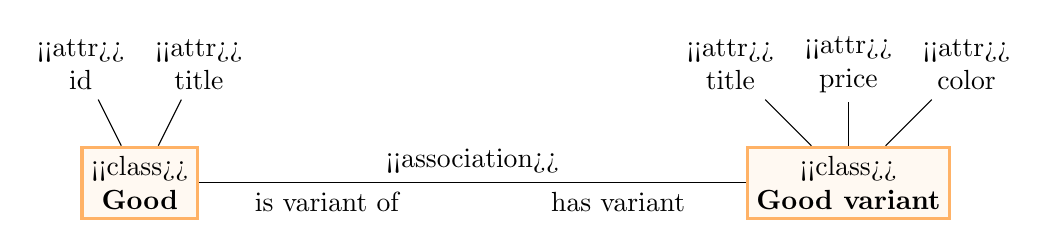
\begin{tikzpicture}[
    class/.style={shape=rectangle, draw=orange!60, fill=orange!5, very thick, minimum size=5mm,align=center},
    attribute/.style={align=center},
  ]
    \node[class] (good) at (0,0) {<<class>>\\\textbf{Good}};
    \node[class] (variant) at (9,0) {<<class>>\\\textbf{Good variant}};

    \node[attribute] (a11) at (-.75,1.5) {<<attr>>\\id};
    \node[attribute] (a12) at (.75,1.5) {<<attr>>\\title};

    \node[attribute] (a21) at (7.5,1.5) {<<attr>>\\title};
    \node[attribute] (a22) at (9,1.5) {<<attr>>\\price};
    \node[attribute] (a23) at (10.5,1.5) {<<attr>>\\color};

    \draw (good) -- (a11);
    \draw (good) -- (a12);

    \draw (variant) -- (a21);
    \draw (variant) -- (a22);
    \draw (variant) -- (a23);

    \draw (good) -- node[pos=0.225,below]{$\blacktriangleleft$ is variant of} node[above]{<<association>>} node[pos=0.775,below]{has variant $\blacktriangleright$} (variant);
  \end{tikzpicture}

  \caption{Schematic diagram of an ontology which could be used for the schema from the \autoref{analysis/general-schema-representation}.}
\end{figure}

% todo popis, jak by mela ontologie vypadat na zaklade toho schematu. Jakou by mela mit strukturu a co musi obsahovat

% mozna ze to je jak uml

\section{Data modeling analysis}

\subsection{Type coherency}

As already mentioned, an ontology is not just a supporting source for the modeling process but rather the only source we can use to create schemas. The schema then represents a mapping to the ontology for further processing.

Because the parts of the schema are mapped, we can check whether the attributes and associations do belong to the given class. This allows us to check, whether the schema is being built correctly and provide the appropriate help during the modeling based on the type of the classes.

Although it may seem that the problem is trivial, there are advanced scenarios that need to be considered.

\begin{enumerate}
  \item We may want to add additional attributes and associations directly into the schema without a connection to the ontology. This is a schema-modeling problem as we may need, for example, to wrap several properties into an additional object (JSON) or a tag (XML) or add another property because the data we validate contains it.
  \item If we have class $A$ in association with $B$ and we have schema with the class $A$ having $B$, then it may be possible to move attributes from $A$ into $B$. Because for each $B$ we know to which $A$ it belongs, we do not loose any information during this process.
\end{enumerate}

As an example of the second case, suppose our ontology has \textit{Goods} and their \textit{Variants}. Variants are colors, sizes, materials, etc., for the given good. Surely all variants are made by one manufacturer. Therefore, it makes sense that the \textit{manufacturer} attribute would be associated with the \textit{Goods} class, whether the \textit{color} with the \textit{Variants}. This may not be beneficiary for all data consumers. Hence a schema with the \textit{manufacturer} attribute moved into the \textit{Variants} class would be a better solution.

\begin{figure}[h!]\centering
  \begin{subfigure}[b]{.5\textwidth}
    \begin{Verbatim}[commandchars=\\\{\}]
\{
  "title": "Chair",
  "variants": [
    \{
      "price": 200,
      "color": "black",
      {\color{red!60}"manufacturer": "IKEA"}
    \}
  ]
\}
    \end{Verbatim}
  \end{subfigure}%
  \begin{subfigure}[b]{.5\textwidth}
    \begin{Verbatim}[commandchars=\\\{\}]
\{
  "customerId": "12",
  {\color{gray!60}"personal-info": \{}
    "name": "John",
    "surname": "Doe"
  {\color{gray!60}\},}
  {\color{gray!60}"contact-info": \{}
    "address": ...,
    "phone": ...
  {\color{gray!60}\}}
\}
    \end{Verbatim}
    \end{subfigure}%
  \caption{Examples of data with some attributes moved. The former moves attribute \textit{manufacturer} from the parent into the other class that has a counterpart in the ontology. The latter takes attributes such as \textit{name} and \textit{address} and wraps them with additional objects that do not correspond to the ontology.}
\end{figure}

This, however, is too complex for the current state of development, but it gives us a chance to think about the problem in a more general way.

\subsection{Data modeling process}

So far, we have only described the desired structure of an ontology and a schema model, but we did not tackle the actual process of how the schema is created.

A user shall start by selecting a root of the schema. Schema under the given root would then describe one entity of the given type, or a list of those entities, depending on the later configuration. Because a set of possible root classes is not limited in any way, the most suitable option is to let user search for the class by its name, descriptions, or other parameters, depending on the given ontology format.

As soon the root is placed in the schema, we get a context because the following attributes and associations to other classes depend on the class where the properties are being added. For that, we use a prompt dialog where it is possible to select those properties to be added.

Although we did not enforce that an ontology must support inheritance, most of them do. Therefore the dialog also allows adding properties of the parent class.

\medskip

The process of adding properties can be more automated in the future. The tool can propose to automatically add all attributes and associations with non-zero cardinality, as it may be the desired behavior, we can perform this action even recursively to automatically design the whole schema just from the root and select a few options where the recursion shall stop. % not a requirement

\bigskip

\begin{requirement}
    The application shall create supporting documents for the generated schemas.
\end{requirement}

The main goal of the tool is to model schemas from a given ontology. Nevertheless, to better understand the generated schema, the documentation, possibly with diagrams and examples, is very beneficial.

A structure of the documentation was already described in the introductory chapter and can be easily derived, as it only describes used concepts that are mapped from the schema.

Regarding examples, for the schema in \autoref{analysis/general-schema-representation}, Figures \ref{analysis/xml-json} and \ref{analysis/csv} could be automatically generated. This would require additional knowledge from the ontology as the application needs to understand that the title should be a buyable item and the price should correspond to the item's actual price.

\section{Data transformations}

\begin{requirement}
    The application shall support generating transformations between different data conforming to supported schemas and RDF representation.
    \label{req:transformations}
\end{requirement}

Data transformations were also introduced at the beginning of this thesis as the necessity for the latter use case of interoperability of public institutions. Data transformations are generally used to convert data (not schemas, but data that conform to given schemas) from one schema to another without changing its meaning.

One example may be to convert CSV to a JSON array of objects, where each object represents a row in the CSV. There are plenty of online tools to do this, but they do not understand the context of the data. Because both schemas were derived from one general schema in the tool, we may correctly map columns from CSV to the fields in a JSON object, not necessarily from a single-table CSV schema.

In the context of this tool, transformation means both (i) transformation between different schemas under the same general schema and (ii) between different general schemas, if possible (as we may exploit the knowledge of the mapping to the original ontology). As an example of the second case, we may have two general schemas for the same thing, where one is simpler than the other. For example, suppose the schema from \autoref{analysis/general-schema-representation} and similar with more attributes and associations, possibly with a different order of properties and labels. It is then possible to convert the data from the more complex schema to the simpler one by losing the information. If default values are provided or additional properties are optional, the transformation in the other direction should also be possible.

\medskip

Regarding the transformation process, there are plenty of ways to transform the data:
\begin{enumerate}
    \item Data engineers use \textbf{Python} with support for many formats using libraries. In this case, the transformation would mean a generated Python script with a predefined interface that takes data from one format and outputs in another. Depending on the use case, the script may be configurable (besides the possibility to configure the generation of transformation itself).
    \item There is \textbf{XSLT} (Extensible Stylesheet Language Transformations) language to transform between XML documents or from XML to XML-like, plain-text, or CSV documents. XSLT is an XML document that can be executed with an input document by an XSLT processor, producing the resulting document. A disadvantage is that the input document must be in XML format; hence, it cannot be used alone for bidirectional JSON and CSV transformation.
    \item There are mapping tools and languages, such as \textbf{RML} \cite{dimou2014rml} (RDF Mapping Language), designed explicitly for mapping purposes. RML maps common serialization frameworks, such as XML, CSV, and JSON, to RDF from a set of rules written in RDF. The translation mechanism is similar to the XSLT. Specifically for JSON, there is \textbf{JSON-LD} with simple directions to set mapping to RDF. Conversion tools are available in multiple programming languages. There is \textbf{CSVW}\footnote{\url{https://csvw.org/}} for CSV as an alternative to the previously mentioned JSON-LD.
\end{enumerate}

Although RML is a ready-to-use solution with support for all three technologies, it requires its own transformation toolchain. This is also valid for JSON-LD and CSVW technologies. On the contrary, XSLT is a well-known technology among people working with XML and is widely supported. Our primary goal is to have transformations that are easy for stakeholders to use in their systems. Therefore, we will implement XSLT for XML while keeping RML for later.

Similar to the translation of a human text, there are two approaches. Either create a transformation for each pair or have one standard format where all the others can be transformed and vice versa. The latter method requires only one transformation for each new format added and is easier to debug, as there is a middle format. Because schemas are built from ontologies whose primary source is RDF, we will exploit this and have RDF as the middle format, which is another format in which we can transform data.

\medskip

We categorize two types of transformation, lifting and lowering. Lifting is a process of converting semi-structured data such as JSON, XML, or CSV into RDF. Lowering is the opposite process. By combining them, we can achieve a transformation between various formats. That means that even if we want to transform XML to CSV, which would be possible by a single XSLT document for simple structures, we would need to execute two transformations.

\begin{figure}[h!]\centering
    \begin{tikzpicture}
        %Nodes
        \node[ontology] (ontology) at (0,0) {Ontology};

        \node[document,align=center] (rdf) at (3,-1.5) {RDF documents};

        \node[generalSchema,align=center] (schema1) at (-3,-1.5) {General\\schema};

        \node[schema,align=center] (xml1) at (-4,-3) {XML\\schema};
        \node[schema,align=center] (json1) at (-2,-3) {JSON\\schema};

        \node[document,align=center] (xml_document) at (1.5,-3.5) {XML\\document};
        \node[document,align=center] (json_document) at (4.5,-3.5) {JSON\\document};

        \draw[-latex] (rdf) -- node[above,anchor=south west,align=left] {conforms} (ontology);

        \draw[-latex] (ontology) -- (schema1);
        \draw[-latex] (schema1) -- (xml1);
        \draw[-latex] (schema1) -- (json1);
        \draw[-latex] (xml_document) to[bend left] node[below] {conforms} (xml1);
        \draw[-latex] (json_document) to[bend left] node[below] {conforms} (json1);

        \draw [->,line width=1pt, transform canvas={xshift=-1.25em}] (xml_document) -- (rdf);
        \draw [->,line width=1pt, transform canvas={xshift=-0.5em}] (rdf) -- (xml_document);

        \draw [->,line width=1pt, transform canvas={xshift=0.5em}] (json_document) -- (rdf);
        \draw [->,line width=1pt, transform canvas={xshift=1.25em}] (rdf) -- (json_document);

        \node[rectangle,fill=white] at (3,-2.35) {lifting and lowering};
    \end{tikzpicture}
    \caption{Example of data transformation. An XML document that conforms to XML schema may be lifted to RDF representation, which conforms to the ontology. The RDF can then be lowered to another format.}
\end{figure}

\section{Data specification}

The following requirements urge us to group similar general schemas into a project that we call a \textbf{data specification}. Schemas in the data specification may share some configuration or depend on each other, as we specify later. Each schema belongs to exactly one data specification. We will not determine in this thesis which schemas should share a data specification and which should not because there are currently no limitations that would state otherwise. However, this may change in the future as new requirements arise.

\begin{requirement}
  It shall be possible to refer to other schemas to use them as building blocks for larger ones. Schema reference shall be treated as a reference to the resulting schemas and documentation as well.
  \label{analysis/requirement/schema-reference}
\end{requirement}

Referencing other schemas is crucial for advanced use-cases where it is essential to split large schemas into smaller blocks that can be published and used separately.

For most schema languages, it should be sufficient to refer to the other schema as is. For example, in JSON, we can use the \verb|$ref| keyword with a path to the referenced schema. On the other hand, data transformations may not always be able to handle this approach. Hence, having a full copy of the schema might be necessary. Referencing a schema would thus require access to all data in its specification.

To avoid problems with tracking references and knowing which data specification needs to be loaded to generate artifacts properly, a user would need to explicitly set a given \textbf{data specification is being reused}. Similarly to the requirement with the ontology, we do not require that the reused data specification be always available.\footnote{See the requirement X for context.} The application shall work even if the data specification is not available at the moment if the presence of the specification is not required directly, such as for creating a new reference or generating artifacts that depend on it.

\begin{figure}[h!]\centering
  \begin{tikzpicture}
      \node[data-specification,align=center] (ds1) at (-3,0) {Data specification 1};
      \node[data-specification,align=center] (ds2) at (3,0) {Data specification 2};

      \node[general-schema,align=center] (s11) at (-4.5,-1.5) {General\\schema};
      \node[general-schema,align=center] (s12) at (-1.5,-1.5) {General\\schema};
      \node[general-schema,align=center] (s21) at (3,-1.5) {General\\schema};

      \draw[-latex] (ds1) -- (s11);
      \draw[-latex] (ds1) -- (s12);
      \draw[-latex] (ds2) -- (s21);

      \draw[-latex,densely dotted] (ds1) -- node[above] {reuses} (ds2);
      \draw[-latex,densely dotted] (s12) -- node[above] {refers} (s21);
  \end{tikzpicture}
  \caption{Example of reusing of specifications. All schemas from reused specification become available to refer from local schemas. Only the root of the schema may be refered.}
\end{figure}

\begin{requirement}
  List of supported schemas, transformations, documents, and other files generated from the general schema shall be easily expandable so that the application can be adapted to different use-cases.
\end{requirement}

Generation of schemas is robust enough to be used in every common scenario, therefore we do not expect that user may want to intervene the process besides the standart configuration, such as indentation, using of comments, or a default language.

On the other hand, documentation is very vague concept that neither we have properly specified. Sometimes a simple Markdown documentation may be sufficient, while elsewhere user may require a strict format of multiple documents in HTML.

Transformations have similar issue. There are multiple ways and technologies that transform data between different schemas. We have already mentioned transformation throught RDF format, either by RML, or custom scripts, such as XSLT for XML. For more demanding user, it is even possible to create transformation scripts between pairs of technology, such as between XML and CSV.

We will expose a way user can register his/her own generator that can create a set of files in a filesystem from the given schema.

Generators may use others to modify their results, further expends them, or just link them.
% Pozadavek na OFN?

\section*{Artifacts}

There is little difference between generated schemas, data transformations, documentation, and other output files. Based on the general schema and provided configuration, if any, the application shall create a set of files that can either be published on the Web or stored in the file system. All the generated files will be denoted as \textbf{artifacts} and are created by the \textbf{generators}.

We will distinguish two types of artifacts. (i) The \textbf{specification artifacts} does not depend on a concrete schema but uses the whole specification. Documentation may be an example of a specification artifact because it generates a single document concerning all the schemas. Of course, this still depends on user requirements, and scheme-specific documentation is possible. (ii) The \textbf{schema artifacts} are bound to concrete general schema and are used to generate transformations or the schema documents.

Artifacts may reference other artifacts. For example, documentation may be the front page of the whole structure, having links to other documents, schemas, images, etc.

\begin{figure}[h!]\centering
  \begin{tikzpicture}
      \node[data-specification,align=center] (ds1) at (-3,0) {Data specification};

      \node[general-schema,align=center] (s11) at (-4.5,-1.5) {General\\schema};
      \node[general-schema,align=center] (s12) at (-1.5,-1.5) {General\\schema};

      \node[artefact,align=center,cascaded] (sa1) at (-7.5,-1.5) {Specification\\artefacts};

      \node[artefact,align=center,cascaded] (sa11) at (-4.5,-3) {Schema\\artefacts};
      \node[artefact,align=center,cascaded] (sa12) at (-1.5,-3) {Schema\\artefacts};

      \draw[-latex] (ds1) -- (s11);
      \draw[-latex] (ds1) -- (s12);
      \draw[-latex] (ds1) -- (sa1);

      \draw[-latex] (s11) -- (sa11);
      \draw[-latex] (s12) -- (sa12);
  \end{tikzpicture}
  \caption{Schemas, documentation, and other generated files are artefacts. Artefact are either schema-specific, that are generated for every schema, or specification-specific for a given data specification.}
\end{figure}

% Necaskeho pozadavek na OR a hierarchii
% https://github.com/mff-uk/dataspecer/issues/95

\begin{requirement}
    It shall be possible to easily add more specific classes to the general schema that extends the base class in a way that data, that conforms the resulting schemas, may contain either the base class, or one of its specialization.
\end{requirement}

\begin{showcase}
    We will start directly with an example. Suppose, that the warehouse also distributes foods besides the general goods. Food is of course type of good, but for storing purposes, it may have additional attributes, such as \textit{storing temperature}. When designing a schema that contains goods anywhere


\end{showcase}

This requirement impacts the application on two different levels. First, the general schema model has to have constructs to represent the required problem and all generators shall understand them and generate a schema that corresponds to the intended result.

Generaly speaking, inheritance is a complex concept, that can be expressed in more simple way. Unfortunatelly, to make this pleasible for a user, we need to represent some things % such as association to class

% Analyza co vsechno se da udelat, co bude privetive a co ne. Rozeberu to na zakladni OR a include.


\chapter{Future requirements}\label{chapters:future-requirements}

The following requirements in this section are analyzed because they may affect the final model that will be discussed in the next chapter. But due to its complexity, full implementation and analysis will be kept as authors' future work and this thesis covers only the necessity to not introduce a technical debt. The requirements follow the authors' intention of creating a whole ecosystem that supports advanced features of sharing and managing schemas.

\section{Ontology modifications}
\begin{requirement}
  \label{requirement:pim-editing}
  The approach from previous tools of creating the ontology directly in the application is not required, but there should be support for \textit{some} modifications.
\end{requirement}

As stated in the \autoref{requirement:ontologies-on-the-web}, the preferred way is to create a complete ontology externally and keep it up-to-date and valid against the requirements of all involved parties.

Nevertheless, there may be scenarios when it may be beneficial to change the ontology directly. Some of them are the following:

\begin{enumerate}
  \item The ontology is wrong and does not describe the domain correctly. - \textit{Then, a correct way would be to fix the ontology.}
  \item The ontology describes only a subset of the domain. Either only the core of the domain or the ontology is complete, but only for one domain, whether in another, something may be missing. - \textit{If the desired ontology is strictly a superset of the domain, we can exploit the linked data features to add missing annotations in our own structured data. Then, we would use the new ontology.}
  \item The ontology is not granular enough. Some entities can be represented in more detail than they currently are or vice versa. - \textit{We would need to create a copy of affected classes or use an advanced tool if it exists.}
\end{enumerate}

Suppose the example with goods in the delivery company. Although the goods may be identified by EAN (barcode on items), the software team may prefer their own internal identifiers. There can be reasons for not including the identifier in the ontology, as it is too specific for only a software team, for example. This would correspond to the second category from the list above. The missing attribute then may belong to either the original class or the new extended class. The third category may represent the case when we, for example, need to replace an address with a set of more specific attributes such as \textit{street}, \textit{number}, \textit{city}, \textit{country}, etc.

Although in all the scenarios, the preferred way would be to create a new ontology or modify the remaining, it can be too cumbersome and time-consuming, especially if the change is too small or the data modeler is performing an experiment. Therefore, the possibility of modifying the ontology should be possible.

But, it may be hard to follow the rules, especially when doing experiments, or small errors need to be fixed.

Allowing such changes must be made carefully, as it may interfere with some mechanisms.
\begin{enumerate}
  \item If the ontology changes, the local overwrites may need to be changed as well, otherwise may become invalid. Overwritten data may get removed or moved elsewhere. Evolution mechanism hence must work with the overwrites as well.
  \item Moreover, the overwriten data may change, which can lead to two scenarios. Either user wishes to keep the local version as if nothing happend, or he/she may want to discard the local version as the new version fixes the issue that caused the modification in the first place.
\end{enumerate}

This issue is too complex and due to the nature of the requirement, it must be solved directly in the application. We keep the question behind this problem partially open and focus only to simple modifications, as this will cover most use-cases.\footnote{From our specific use-case on the Semantic government vocabulary (SGOV), most of the changes consist of adding a missing cardinality or fixing labels and descriptions.}

\section{Ontology alignments}
\begin{requirement}
    As there shall be a support for data transformations between different schemas, the data transformations shall respect various ontology alignments to transform data between different ontologies. Alignments shall also be created during user modification of the ontology, between the modification and the original ontology.
    \label{requirement:ontology-alignments}
\end{requirement}

\textbf{Alignment}, as defined in \cite{euzenat_ontology_2013} is a set of relations between entities, \textit{usually} from different ontologies. These relations specify the semantic equivalence between them and create a mapping that can be used to transform data from one representation to another.

There are already well-known RDF predicates that can cover basic alignment. For semantically identical entities, we may use \verb|owl:equivalentClass| or \verb|skos:exactMatch|. A more useful RDF predicate is \verb|rdfs:subClassOf| to specify that the given class extends others by specializing its type.

The latter is already used in the previous \autoref{requirement:inheritance}. Subclasses (i) reuse attributes and associations from their parent class but also semantically denote that (ii) the subclass can also be treated as "the parent class." The second point is an example of a simple ontology alignment. In the context of data transformations, we can take the ore specific class and convert it to its base type.

\medskip

As an advanced example, suppose again the address property that is used for delivery purposes. The address can be represented as one multi-line string value or as its parts such as street, number, etc. The most straightforward mapping would split the string by commas and new lines and join them back, respectively.

The user can then decide whether they want to use the first or the second group of entities, and the transformation script would still be able to transform data between those two representations.

\begin{figure}[h!]\centering
  \centering
  \begin{tikzpicture}[
    attribute/.style={align=center},
  ]
    \node[ontologyClass] (ci) at (0,0) {<<class>>\\\textbf{Contact information 1}};

    \node[ontologyClass] (ci2) at (6,0) {<<class>>\\\textbf{Contact information 2}};

    \node[attribute] (a1) at (0,1.5) {<<attr>>\\address};
    \node[attribute] (a2) at (4.5,1.5) {<<attr>>\\street};
    \node[attribute] (a3) at (6,1.5) {<<attr>>\\number};
    \node[attribute] (a4) at (7.5,1.5) {<<attr>>\\city};

    \draw (ci) -- (a1);
    \draw (ci2) -- (a2);
    \draw (ci2) -- (a3);
    \draw (ci2) -- (a4);

    \node[mapping,align=center] (map) at (3,3.5) {<<alignment>>\\\{address\}=\{street\}, \{number\}\textbackslash n\{city\}};

    \draw[-latex] (map) -- (a1);
    \draw[-latex] (map) -- (a2);
    \draw[-latex] (map) -- (a3);
    \draw[-latex] (map) -- (a4);

  \end{tikzpicture}
  \caption{Example of mapping between different representations of address.}
  \label{figure:address-mapping}
\end{figure}

\medskip

The primary purpose of alignments is to use them for better data transformations, as different general schemas may use different parts of the ontology. By connecting them with alignment, we may be able to transform the data between a wider variety of schemas. We shall note that using multiple syntactically different ontologies in modeling is not our use case as our primary focus is to use ontology designed primarily for modeling. Nevertheless, there are some scenarios where some alignments are useful.

In general, we can use alignments directly from various ontologies (see \autoref{requirement:ontologies-on-the-web}) if the ontology supports it. As we have pointed out, we already use subclassing from the supported ontologies.

In addition to explicit use, alignments are also crucial for local modifications (see \autoref{requirement:pim-editing}). As we decide to introduce a new entity or modify others, it will be beneficial to keep the information that those entities are somehow related to the original ontology. Suppose the example with the address. We find that the address as a single field is not sufficient. Therefore, we split the address into individual parts and use them. The alignment together with the transformations still produces valid RDF data according to the original ontology.

This approach can even be used to create transformation scripts between old and new data if the ontology changes (see \autoref{requirement:evolution}). % We would simply instruct the propagation mechanism not to modify the PIM but rather create new entities and keep the old uninterpreted. We would then copy all schemas that were affected and evolute the copies. This would create new schemas and keeps old ones under the same PIM. Semantic mapping with data transformations would then generate the transformation scripts.

%We will keep the question behind the mapping open as it is way too advanced for the current state of the project. However, introducing a new PIM construct to the framework that maps the entities should not collide with the rest of the framework. And as it is at the PIM level, it would be possible to extract this information from CIM.

\section{Evolution}
\begin{requirement}
    It shall be possible to perform a top-down evolution of schemas and other documents from an ontology. The evolution shall be automatic, if possible, and shall also transorm the data that conform the given schemas. The application shall also deduce the changes from an ontology that does not support versioning.
\end{requirement}

Schema evolution is a large topic with many theoreticall issues.

% popis evoluce, priklady

\section{Interoperability}
\begin{requirement}
    The tool shall support working with general schemas that are not directly stored in it but may be located in another instance, on the web, or in Solid Pods\footnote{Solid (\url{https://solidproject.org/}) is a specification for storing data in decentralized places called Pods. Users may create Pods in their own servers or use services that provide that option. It is an alternative to services like Facebook or Google that stores data on their servers only.}.
    \label{requirement:schemas-on-the-web}
\end{requirement}

We have already discussed data on the web principle regarding ontology (see \autoref{requirement:ontologies-on-the-web}), as it is preferred to have data published on the web to be easily accessible by anyone. Although this can be achieved in other ways (such as public API, regular dumps, etc.), the great benefit lies in the fact that those data are independent of the tool that created them. Those data can be easily modified and accessed by other tools (if the given tool understands its structure) and, if necessary, moved under a different database.

Similarly, we would like to achieve this with all data representing the schema's state. Specifically, we mean the structure of the general schema, configuration of all artifacts, other configurations, and helper files. Instead of having an enclosed application that stores all data internally and only provides a way for exporting and importing them, we would like to have ways to read schemas from other sources similarly as they are local and modify them as well if the user is allowed to do so.

This approach allows data modelers to create their own schemas that can be reused by anyone else on the internet. Because the schemas would be hosted by their infrastructure, there is no need for a centralized service that would need to deal with user accounts, GDPR, payments for schema hosting, integration of other tools, etc. Of course, this also means that there would be no repository with search functionality for the schemas.

\medskip

In most cases, storing data externally should not be a problem, as we need to read them from somewhere anyway. If the external storage is inaccessible, the application shall still provide most of its functionality and try to obtain the data later. For example, this may mean that it would not be possible to generate some artifacts, and part of the schema in the UI would not be visible. Because we have introduced data specifications as projects, the problem would only occur when referencing a subschema from a data specification that is stored in the problematic source.

This approach may be challenging if we begin changing the schemas. In the current state of the implementation, schemas can be referenced. If the referenced schema changes (either by evolution or directly by user), the reference may become broken, and referencing schema becomes invalid. In sections \ref{subsection:type-coherency} and \ref{sec:type-coherency} we already tickled type coherency and when schema becomes invalid.

This, together with the fact that schemas may be modified outside the tool, has significant implications as some checks on schemas must be performed continuously and not just during the construction of the schema. Generally, that would mean that schemas may be invalid/broken at any time, and the tool shall still be able to work with them.

\section{Schema inheritance}
\begin{requirement}
    It shall be possible to extend any existing general schema by adding or modifying some of its properties. The extended schema shall remain linked to the original one and allow propagation of changes if the original schema is modified.
    \label{requirement:schema-inheritance}
\end{requirement}

As an example, suppose someone designs and publishes a general schema (not the generated JSON or XML schemas, but the data specification itself).

\begin{itemize}
    \item The most common scenario is to work with data that conforms to the schema as is. For example, the author of the schema publishes the data in one of the formats, and we only need to process them. For this, we only need to generate schemas from the published schema.
    \item An advanced scenario is that we need to wrap the data and send them elsewhere. Hence we need to create a new schema containing the original one. In this case, the schema reference is sufficient as we do not modify the content of the payload. (see \autoref{fig:schema-inheritance:json-data-unaltered})
    \item This requirement addresses a scenario where the payload is somehow modified. For example, we may want to create a proxy server which removes personal information from the payload if the user is not logged in. (see \autoref{fig:schema-inheritance:json-data-censored}) Another examples are to add a timestamp directly to the payload, or add additional information to some parts of the data.
\end{itemize}

\begin{figure}[h!]\centering
  \begin{subfigure}{\textwidth}
  \begin{Verbatim}[commandchars=\\\{\}]
{\color{red!60}\{}
  {\color{red!60}"name": "John Doe",}
  {\color{red!60}"role": "customer",}
  {\color{red!60}"e-mail": "jd@example.com"}
{\color{red!60}\}}
    \end{Verbatim}
    \caption{JSON data that conforms the original schema. (the payload)}
  \end{subfigure}


  \begin{subfigure}[b]{.45\textwidth}

    \begin{Verbatim}[commandchars=\\\{\}]
\{
  "recipientPerson": {\color{red!60}\{}
    {\color{red!60}"name": "John Doe",}
    {\color{red!60}"role": "customer",}
    {\color{red!60}"e-mail": "jd@example.com"}
  {\color{red!60}\}},
  "message": "Summer sale!"
\}
    \end{Verbatim}
    \caption{JSON data that contains unaltered payload.}
    \label{fig:schema-inheritance:json-data-unaltered}
  \end{subfigure}\hfill%
  \begin{subfigure}[b]{.45\textwidth}
    \begin{Verbatim}[commandchars=\\\{\}]
{\color{red!60}\{}
  {\color{red!60}"name": "John Doe",}
  {\color{red!60}"role": "customer",}
  {\color{red!60}"e-mail": null}
{\color{red!60}\}}
    \end{Verbatim}
    \caption{JSON data of the payload with censored {\tt e-mail} as it is the personal information.}
    \label{fig:schema-inheritance:json-data-censored}
    \end{subfigure}%
  \caption{Example of the second and third scenario from \autoref{requirement:schema-inheritance}.}
\end{figure}

